\documentclass[12pt]{beamer}
%\documentclass[20pt,handout]{beamer}
\usetheme{Darmstadt}
\usepackage{graphicx}
%\usepackage[german]{babel}
\usepackage[T1]{fontenc}
\usepackage[utf8]{inputenc}
\usepackage{tikz}
\setbeamertemplate{footline}[frame number]

\newcommand{\cc}[1]{\includegraphics[height=4mm]{img/#1.png}}
\usepackage{ifthen}
\newcommand{\license}[2][]{\\#2\ifthenelse{\equal{#1}{}}{}{\\\scriptsize\url{#1}}}
\usepackage{textcomp}

\pgfdeclareimage[height=.6cm]{c3d2logo}{./img/c3d2.pdf} 


\pgfdeclarelayer{foreground}
\pgfsetlayers{main,foreground}
\logo{\pgfputat{\pgfxy(-1,0)}{\pgfbox[center,base]{\pgfuseimage{c3d2logo}}}}


\title{CMS-Einführung}
\author{\small Paul Schwanse\\\large Chaos Computer Club Dresden}
\date{07.04.2014}

\begin{document}
\maketitle

\section{Einleitung}
\subsection{}

\begin{frame}
  \frametitle{Hacker}
  \begin{figure}
    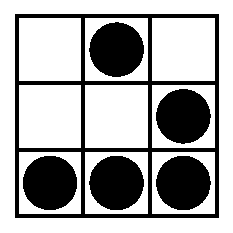
\includegraphics[height=0.7\textheight]{img/Glider.pdf}
  \end{figure}
\end{frame}
\end{document}
